
% \documentclass[10pt]{article}
\documentclass[10pt,twocolumn]{article}
\setlength\columnsep{6mm}

\usepackage[english]{babel}
\usepackage[stretch=10, shrink=10]{microtype}
% \usepackage[a4paper]{geometry}
\usepackage[a4paper, total={6.5in, 9in}]{geometry}
\usepackage{caption}
\usepackage{subcaption}
\usepackage{amsmath}
\usepackage{multirow}
\usepackage{xcolor}
\usepackage{hyperref}
\usepackage{float}
\usepackage[linesnumbered,lined,commentsnumbered]{algorithm2e}
\usepackage{enumitem}
\ifdefined\noimage  % For omitting images during build from CLI
    \usepackage[demo]{graphicx}
\else
    \usepackage{graphicx}
\fi

% Tighter vspace in enumerate/itemize
% \setlist{noitemsep,topsep=0pt,parsep=0pt,partopsep=0pt}

\hypersetup{  % Prevents colored boxes around \cite and \ref
    allbordercolors = {white}
}

\newcommand{\note}[2]{#1${}_{#2}$}
\newcommand{\notesharp}[2]{#1${}_{#2}^{\sharp}$}
\newcommand{\noteflat}[2]{#1${}_{#2}^{\flat}$}

\newcommand{\floor}[1]{\left \lfloor #1 \right \rfloor}
\newcommand{\ceil}[1]{\left \lceil #1 \right \rceil}
\newcommand{\round}[1]{\left \lfloor #1 \right \rceil}


\title{\textbf{Real-time monophonic guitar pitch estimation}\\The feasibility of Fourier transform based methods}
\author{Luc de Jonckheere}
% \date{}

\begin{document}
\selectlanguage{english}

\maketitle


\section*{Abstract}
\textcolor{gray}{Short summary.}


\tableofcontents


\section{Introduction}
Pitch estimation, which is also referred to as f0 estimation, is an important subtask within the field of Automatic Music Transcription (AMT). The goal of pitch estimation is to estimate the pitch or fundamental frequency $f_0$ of a given signal. In the context of AMT, pitch estimation is used to determine what note is played in a given signal.

Real-time pitch estimation is a subproblem where we want to estimate the note associated with the measured pitch while the musician is playing it with minimal latency. This entails we have to use the latest received signal. In contrast to non-real-time methods, we have no knowledge of what may happen ahead of time and signal corresponding to previous notes is mostly irrelevant. This limits the methods we can use to solve this problem.

If pitch estimation can accurately be performed in real-time, it can be used to create a digital (MIDI) instrument from an acoustic instrument. This digital instrument can then be used as an input for audio synthesizers, allowing musicians to produce sounds from a wide variety of instruments. Furthermore, accurate real-time pitch estimation can be used to automatically correct detuned instruments by pitch shifting the original signal to the closest harmonious note.

The Fourier transform is often used to decompose a signal into the frequencies that make up the signal. Predominant frequencies in the signal show up as spectral peaks in the frequency domain. These peaks are important to human perception of melody~\cite{hearing}. %The popularity of the Fourier transform in pitch estimation is likely due to its widespread use in
Other popular methods used for pitch estimation include non-negative matrix factorization, autocorrelation, statistical model based estimation and hidden Markov model based estimation.

Our research focusses on monophonic pitch estimation. Here, we assume the signal contains at most one note. It is much easier to perform monophonic pitch estimation compared to polyphonic pitch estimation~\cite{monotopoly}, especially when using Fourier transform based methods, as fundamental limits of the Fourier transform inhibit our ability to discern two low pitched notes~\cite{nopoly}. Furthermore, hexaphonic guitar pickups are becoming more widespread, which allows us to view the guitar as six monophonic instruments instead of one six-way polyphonic instrument. Commercial guitar synthesizer solutions from companies with big research departments such as Roland also use these hexaphonic pick-ups, which indicates the infeasibility of accurate and responsive polyphonic pitch estimation of a guitar.

This thesis builds upon a preliminary research project~\cite{ik}. In our research project, we found that Fourier transform based pitch estimation methods might not be well suited for real-time use due to fundamental limitations of the Fourier transform~\cite{fourierlimit}. In this work, we will further research if Fourier transform based methods are viable, as real-time transcription research often relies Fourier transform based methods.

\textcolor{gray}{TODO: Rewrite this paragraph.} The goal of this thesis is to research the limits of Fourier transform based real-time pitch estimation. To correctly assess the limits, we develop a pitch estimation framework. This framework will focus on extensibility and the ability to perform automated tests. This is important, as much work in this field does not provide its associated source code. This limits the ability to build on other's work and hinders direct comparisons between different methods. Our framework can provide a common ground for the different methods and algorithms to be implemented and compared in. The framework is available at \url{www.github.com/lucmans/digistring}.


\section{Related work}  \label{sec:related}
Much research has been performed on Fourier transform based real-time pitch estimation. All research we found relies on obtaining a high resolution frequency domain in which spectral peaks can be isolated and notes can be associated with. These methods are deemed infeasible by some due to low frequency resolution~\cite{fourierlimit}.%, however, in our research project we found that it might still be possible. The lack of resolution in the low frequencies is especially problematic when adhering to a real-time constraint, as extra short signal frames have to be used.
This is especially problematic when adhering to a real-time constraint, as extra short signal frames have to be used. Some papers circumvent this problem by choosing a very high real-time constraint~\cite{sloomboi, sloomboi2}, however, this inhibits the use for real-world applications. Furthermore, conventional operating systems also have a latency when delivering audio samples to your program due to how audio drivers work~\cite{oslatency}.

A big problem with Fourier based pitch estimation is the occurrence of overtones~\cite{oud}. Especially octaves are a problem, as the fundamental and all overtones of the higher note overlap with overtones of the lower note. This is referred to as the octave problem~
\cite{octave}. Overtones are periodic in nature, as they diminishingly repeat every multiple of the fundamental frequency. As a consequence, they could also be detected using a subsequent Fourier transform~\cite{doublefourier} on the frequency domain. However, this does not solve the octave problem.

Many different transform have been researched for pitch estimation, however, Fourier transform remains popular as it is broadly studied and its behaviour is well known~\cite{survey}. Lately, the CQT transform is gaining popularity as it may provide higher resolution in the frequency domain~\cite{cqtres} at the cost of lower computational efficiency~\cite{cqtslow}. However, the CQT transform is efficiently implemented using Fourier transforms~\cite{cqtfft} and the main problem with Fourier is the fundamentally low frequency resolution on short frames, so we are left with the same problem. One big advantage is that the frequency bins can perfectly align with the notes of an instrument~\cite{cqtalign}. However, as described in Section~\ref{sec:overtones}, overtones are dissonant with respect to our notes and consequently, the CQT bins do not align with the overtones. If a note perfectly aligns with a Fourier bin, all overtones will also align. In order to cover every note, we could instead perform 12 Fourier transform in parallel. This difference is especially important when performing polyphonic transcription.


\section{Preliminaries}
\textcolor{gray}{Jargon required to understand this paper.}

\subsection{Audio processing}
\textcolor{gray}{Audio is represented by samples. We get these samples from the OS audio driver. Driver latency.}

\subsection{Fourier transform}
The Fourier transform is a mathematical transform which transforms a function of time to a complex valued function of frequency and phase. Here, the magnitude represents the amplitude and the argument represents the phase of the corresponding sine wave. The Fourier transform works on continuous functions and assumes an infinite time interval. Concepts such as continuous and infinite cannot be represented by a computer. Consequently, the discrete Fourier transform (DFT) has to be used for Fourier analyses on computers. The DFT can efficiently be calculated using the fast Fourier transform (FFT) algorithm.

The DFT transforms a finite sequence of equally spaced samples, which we will refer to as a frame, into an equal number of complex values representing the amplitude and phase, which we refer to as bins. When working with audio, the samples are real valued, and the DFT output is symmetrical. Because of this, we can discard the second half of the output. In the rest of this thesis, we will only consider the first half of the output. Each bin corresponds to a specific frequency. All other frequencies are spread out over multiple bins due to spectral leakage, which will be discussed later. Given a frame $F$, the number of samples is the frame is $n_F = |F|$. Using $n_F$ and sample rate $f_{\text{SR}}$, we can calculate the distance between bins in Hz:
\[ \Delta f_{bin} = \frac{f_{\text{SR}}}{n_F} \]
This is also referred to as the frequency resolution. Closely related to the frequency resolution is the frame length, which is calculated as follows:
\[ t_F = \frac{n_F}{f_{\text{SR}}} \]
Given a bin number $i \in [0, \floor{\frac{n_F}{2}}]$, the frequency of a bin can be calculated as:
\[ f_{bin} = \Delta f_{bin} * i \]
The 0 Hz bin corresponds to the so called DC offset. This is the average amplitude of the signal. The frequency of the last bin is also called the Nyquist frequency, which is the highest frequency which can be sampled without aliasing. The Nyquist frequency is equal to half the sample rate.

The DFT assumes the frame to be periodic. In other words, the frame is regarded as infinitely repeating. This may lead to aliasing if the beginning and end of a frame do not align, see Figure~\ref{fig:framealias}. Here, we take a frame shown by the red lines. The frame is not aligned to a period of the sine wave and causes aliasing as seen in the second graph. This kind of aliasing is called spectral leakage and causes other frequencies which are not a multiple of $\Delta f_{bin}$ to spread out over multiple bins. By applying a window function, the beginning and end of a frame are forced to align.
\begin{figure}[H]
    \centering
    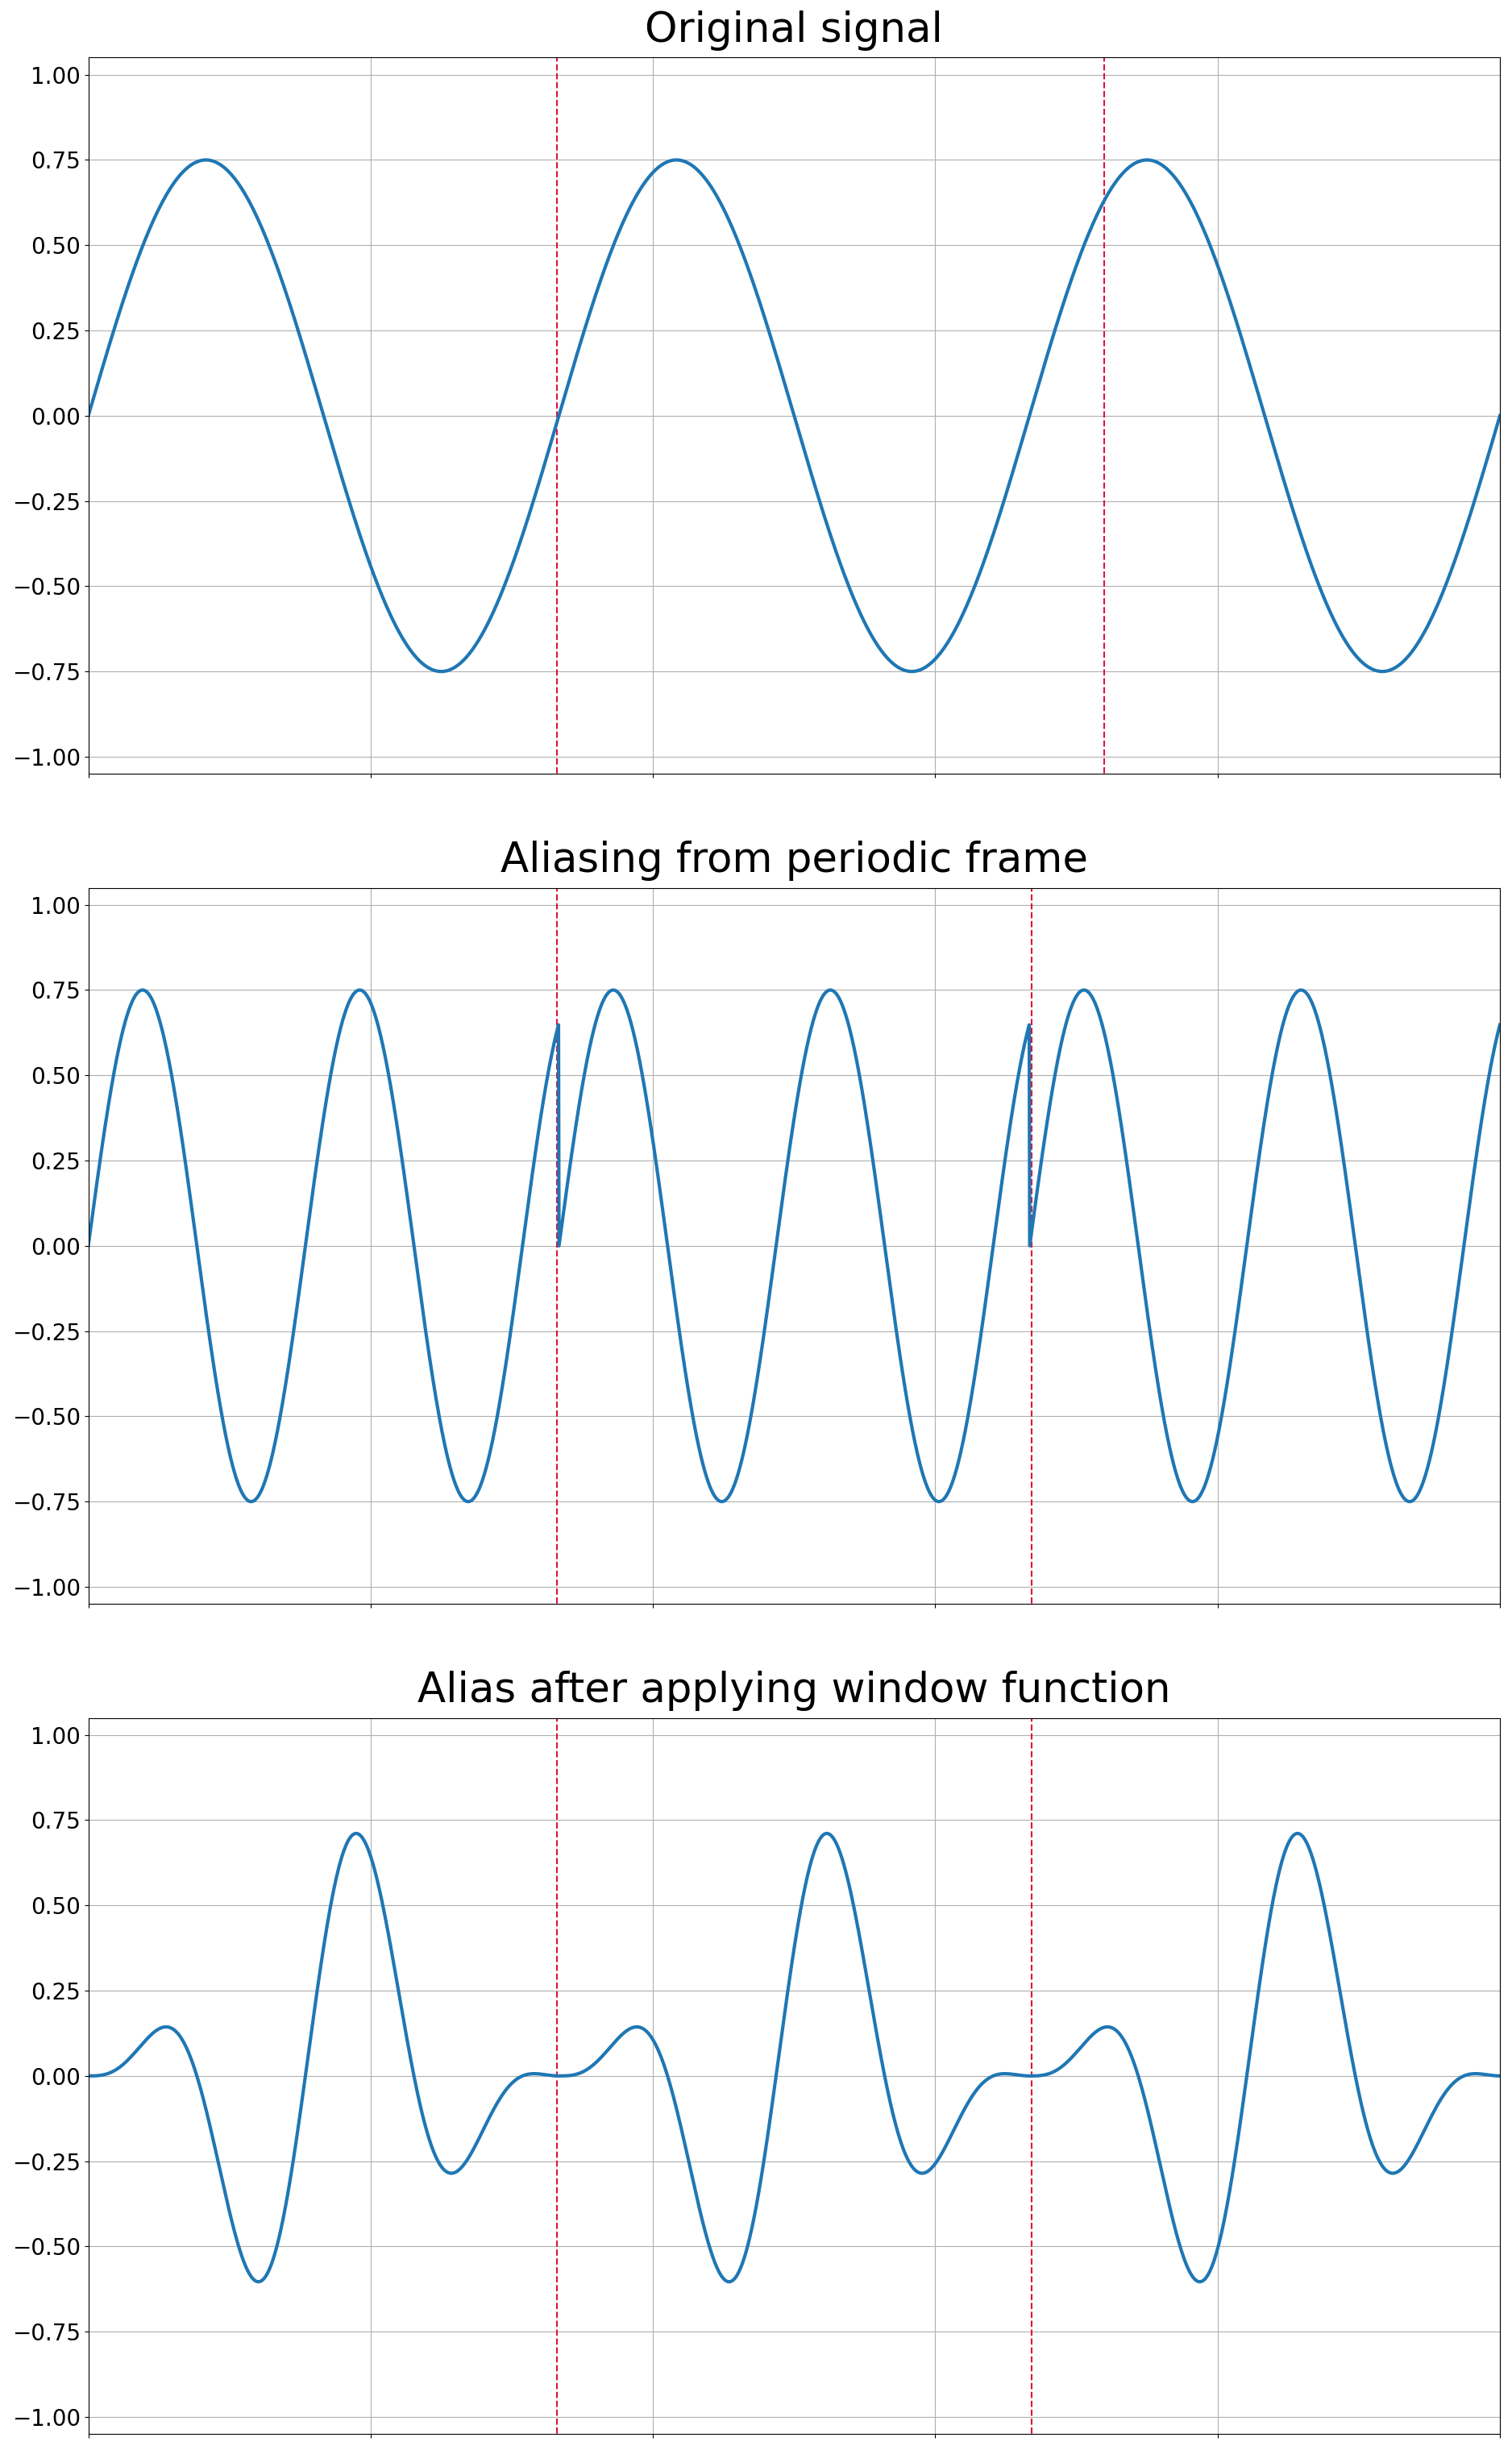
\includegraphics[width=\linewidth]{fig/leakage.png}
    \caption{Aliasing which occurs when performing the discrete Fourier transform}
    \label{fig:framealias}
\end{figure}

Spectral leakage can be controlled using window functions. Given signal $s(n)$ and window function $w(n)$, we get the resulting signal $\text{res}(n)$ using:
\[ \text{res}(n) = s(n) * w(n) \]
Figure~\ref{fig:windowfunc} shows the working of a window function on a frame graphically.
\begin{figure}[H]
    \centering
    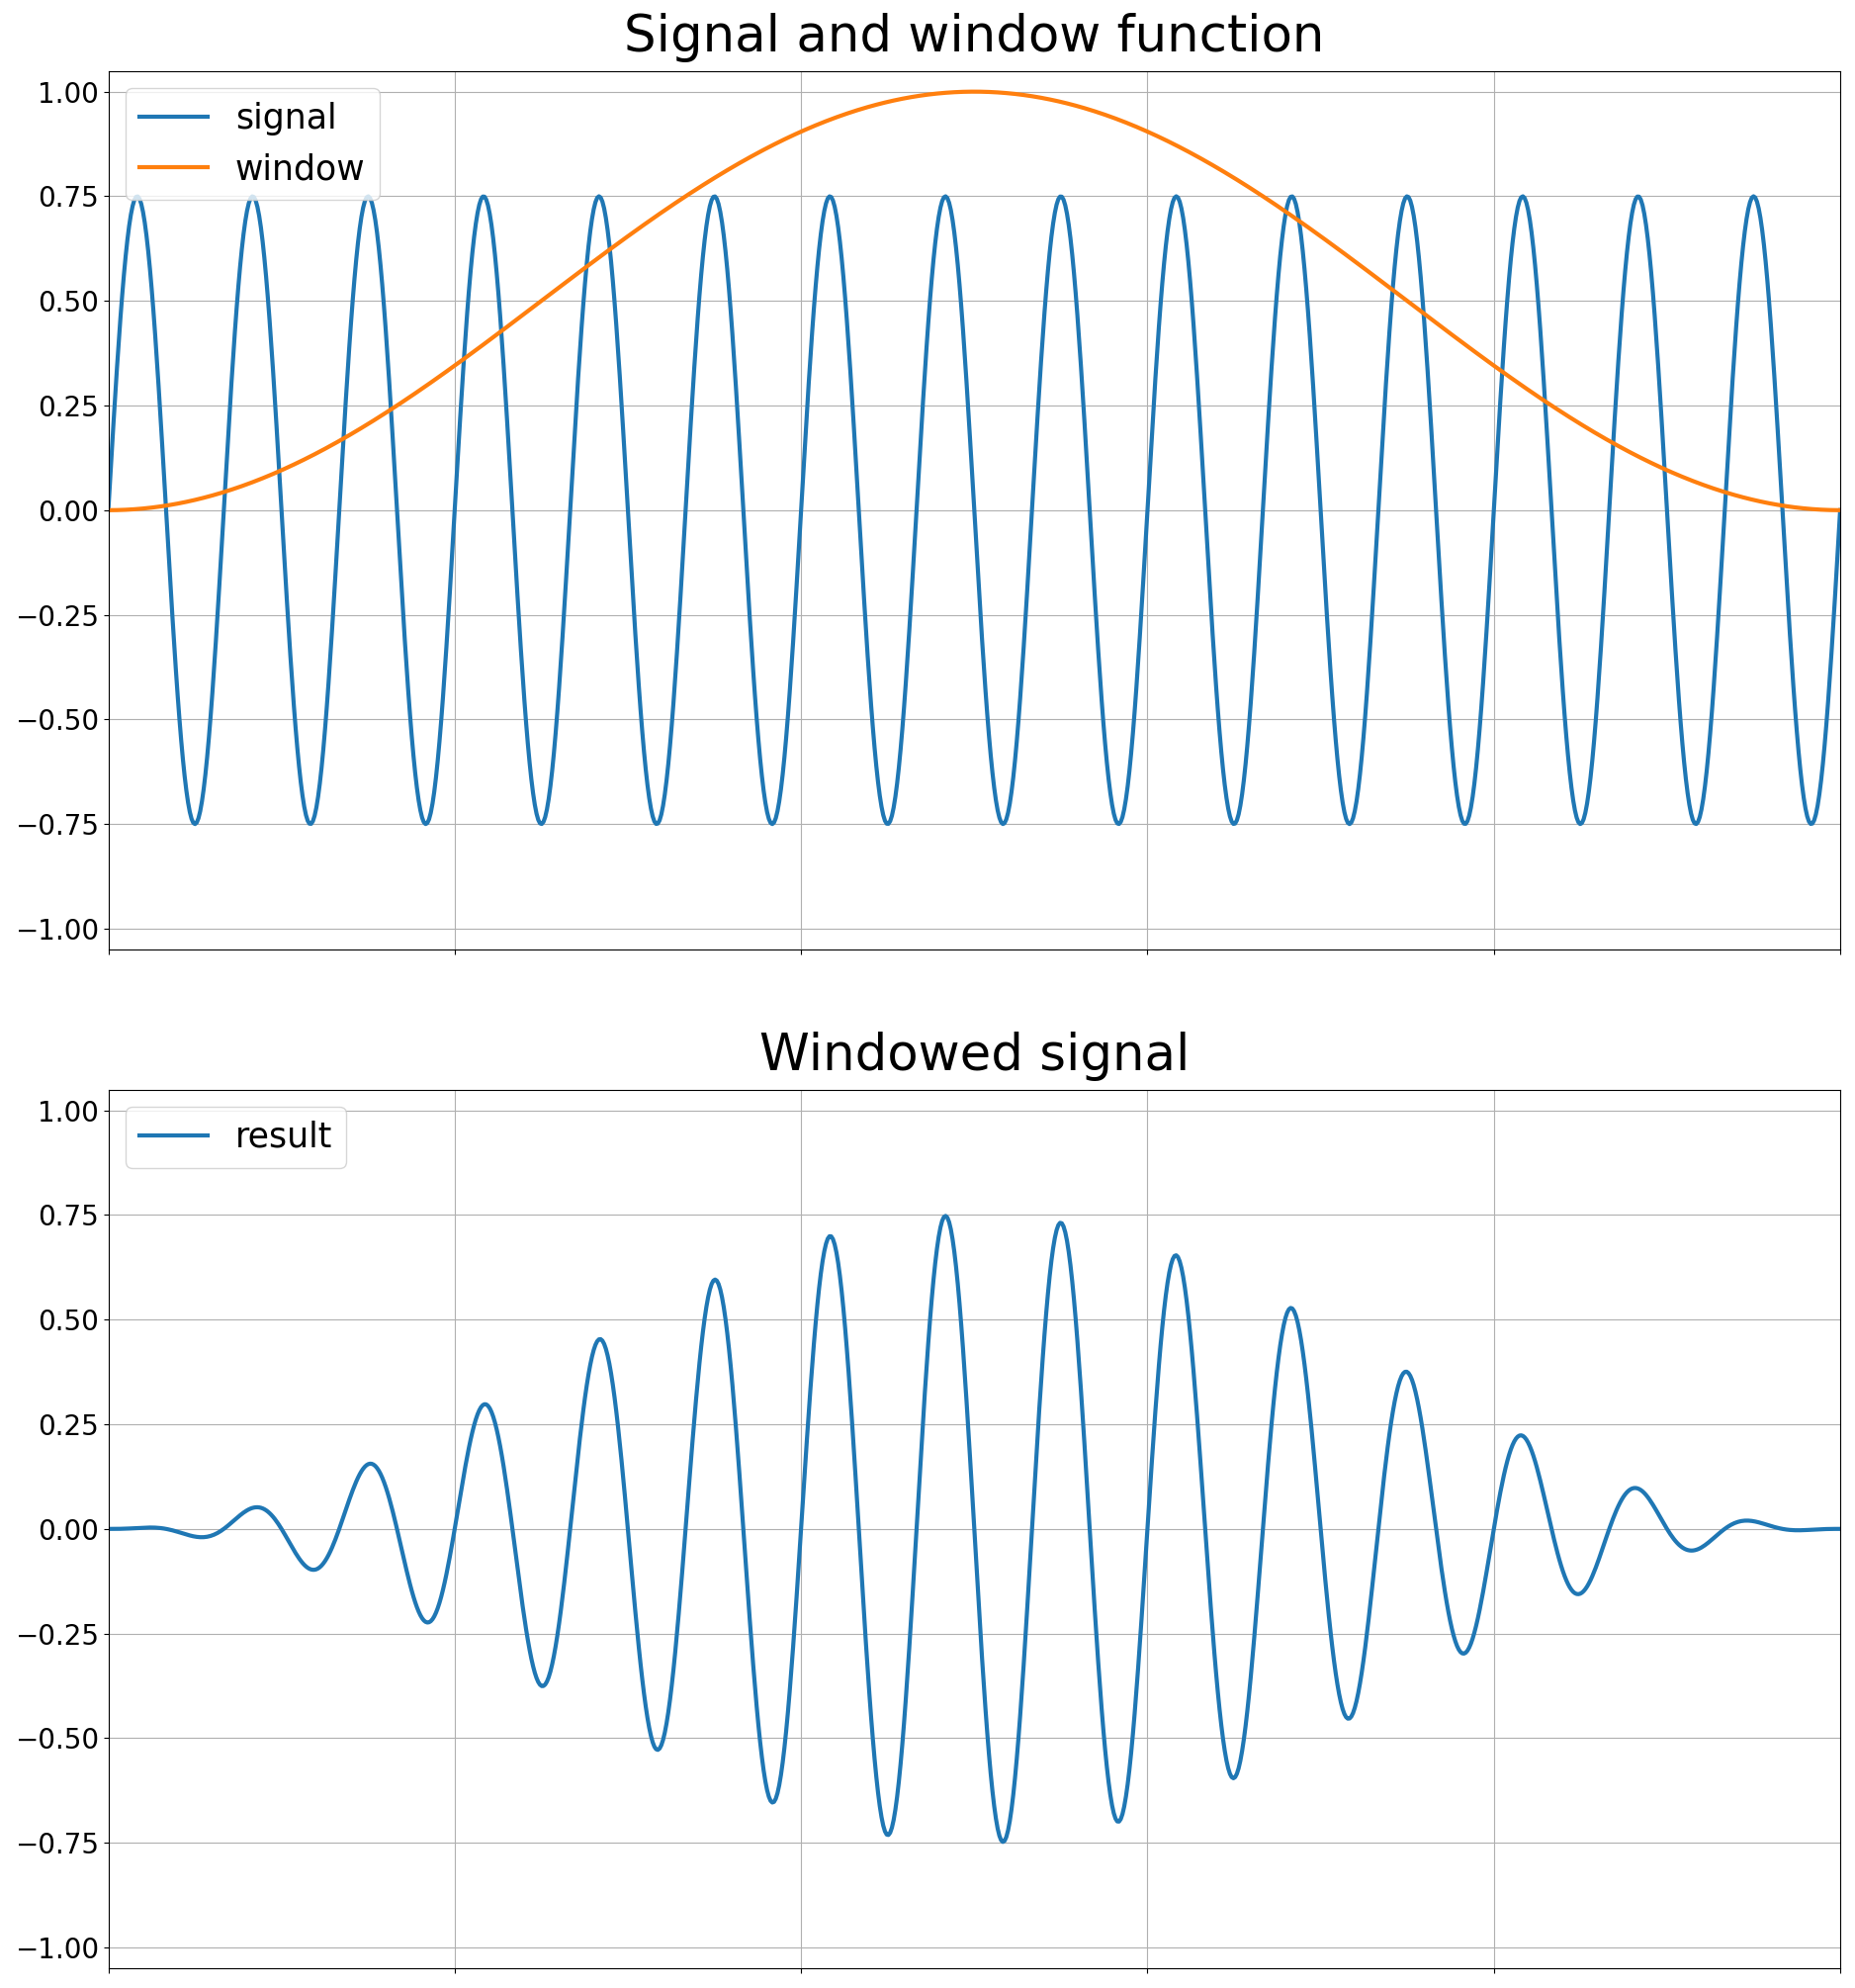
\includegraphics[width=\linewidth]{fig/window.png}
    \caption{An example of using a window function on a signal}
    \label{fig:windowfunc}
\end{figure}
\noindent The different windows functions trade of between a narrow center lobe and little overall leakage~\cite{windowfunc}, see Figure~\ref{fig:windowfunceffect} for some examples. Using the rectangular window could be considered as using no window function. It simply only takes $n_F$ samples from the wave without any alteration. The Hann window is an all round performing window and as a result is often used. The Welch window is a window with a very narrow center lobe. The Dolph–Chebyshev window has little and very evenly spread overall leakage.
\begin{figure}[H]
    \centering
    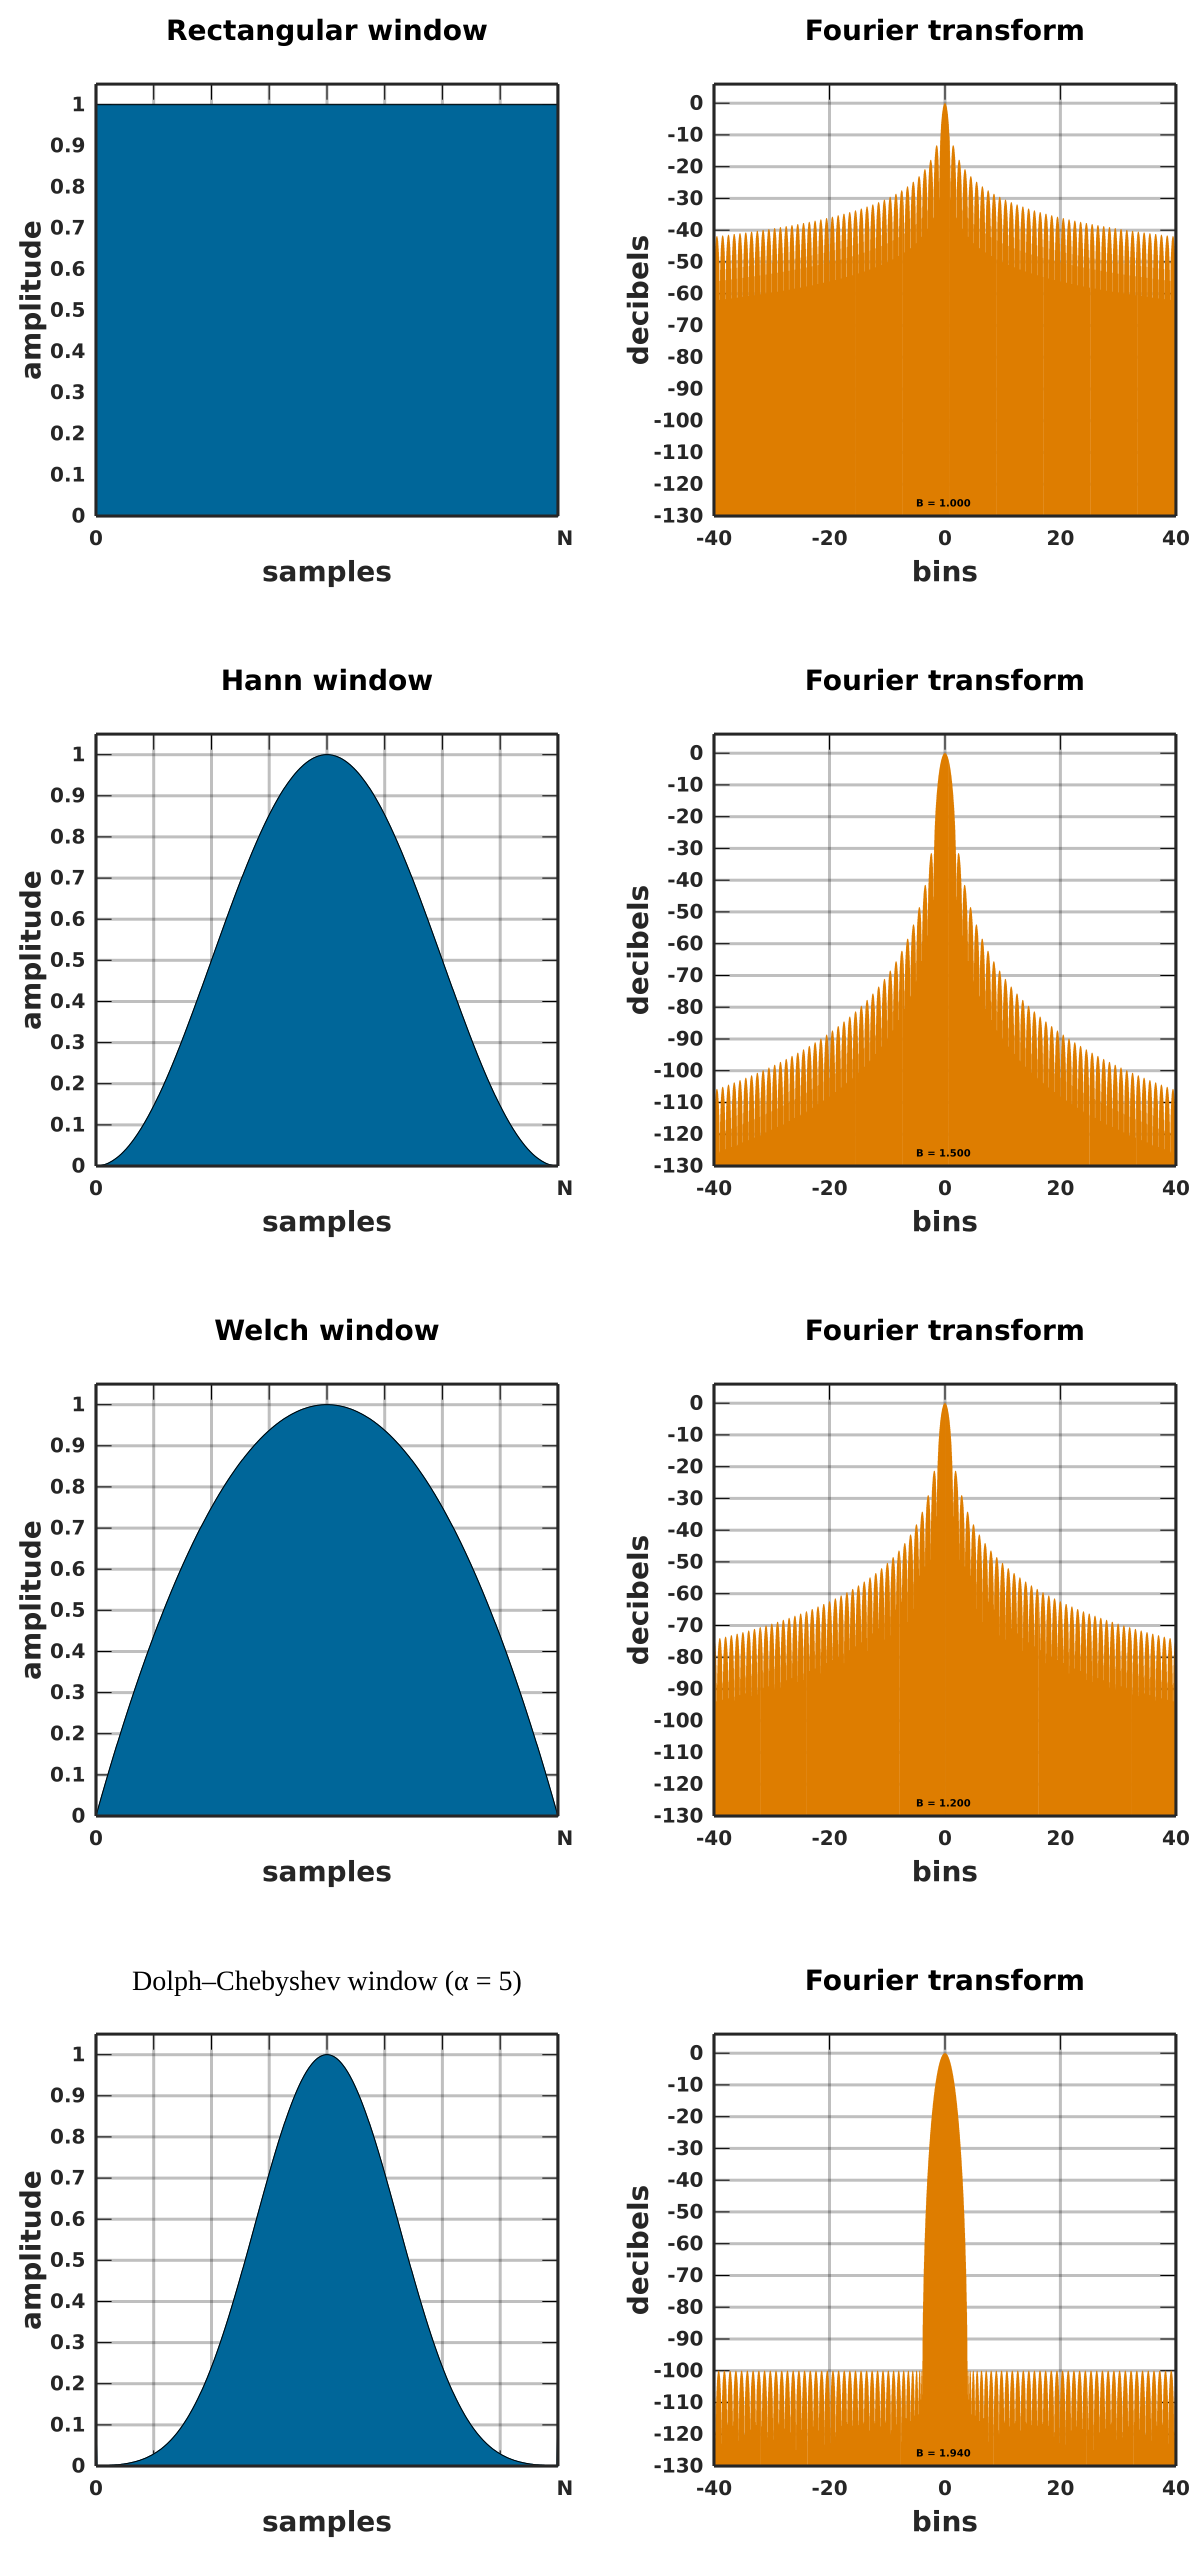
\includegraphics[width=\linewidth]{fig/windows.png}
    % 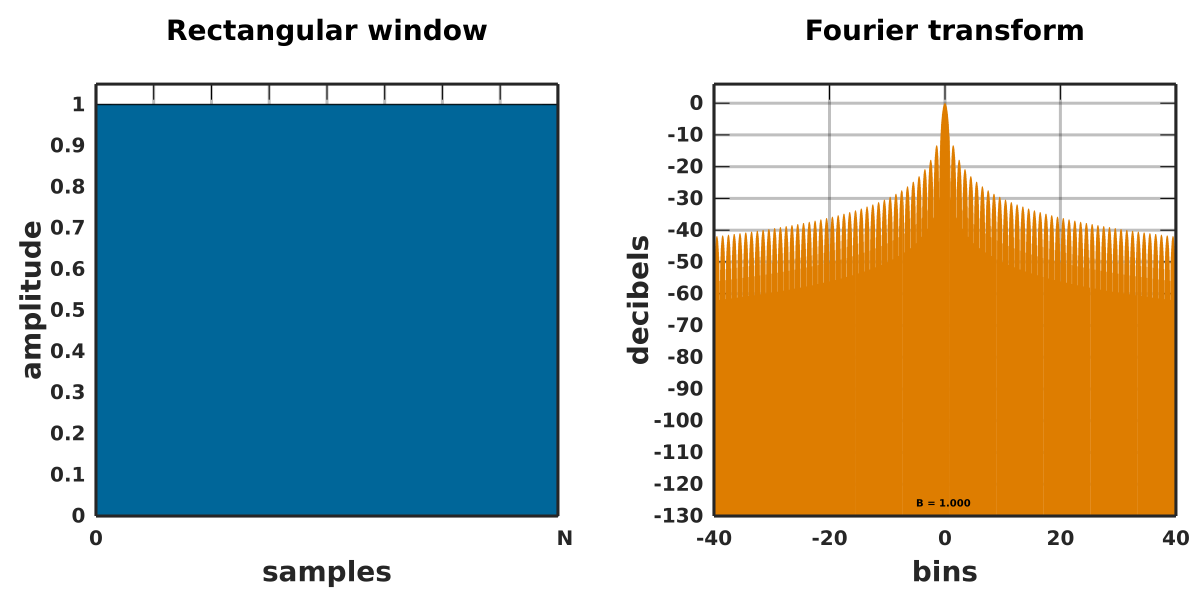
\includegraphics[width=\linewidth]{fig/window_rect.png}
    % 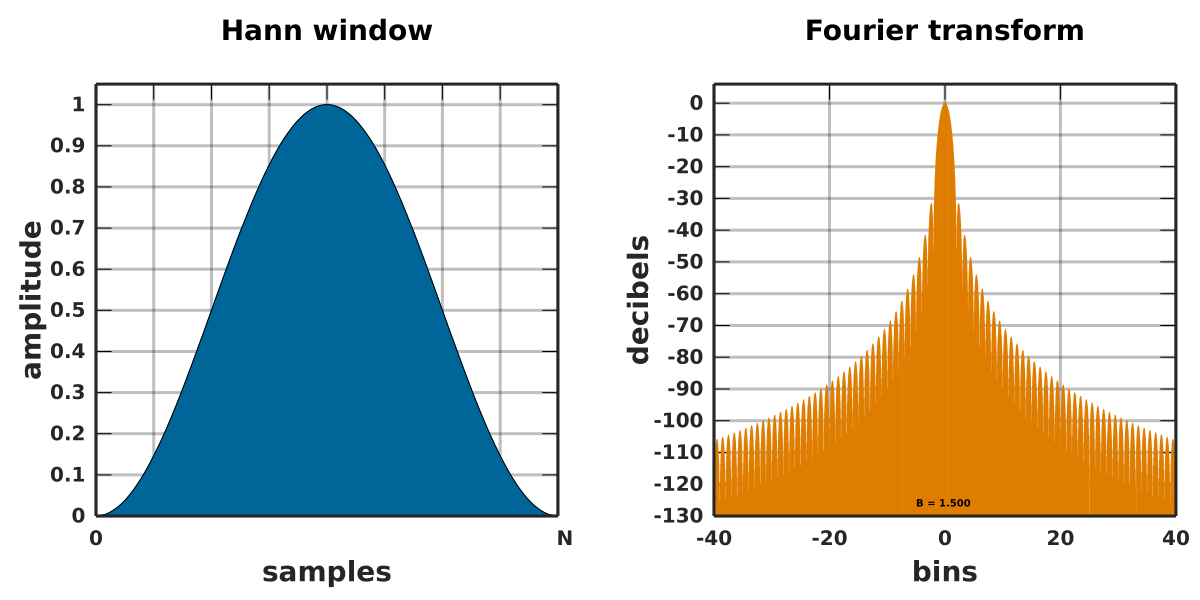
\includegraphics[width=\linewidth]{fig/window_hann.png}
    % 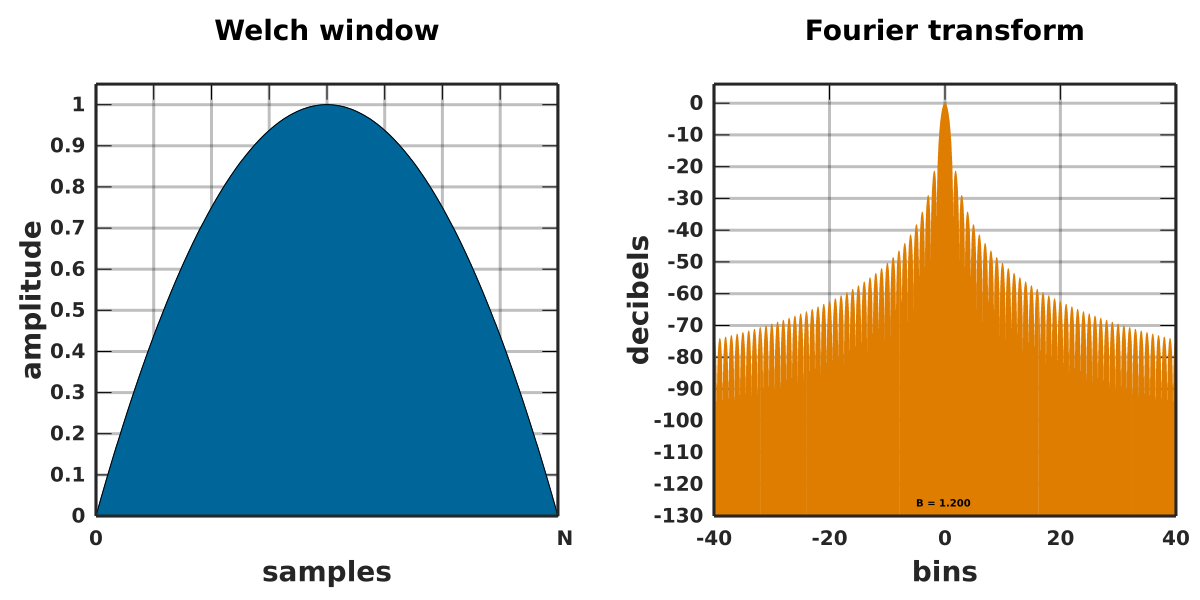
\includegraphics[width=\linewidth]{fig/window_welch.png}
    % 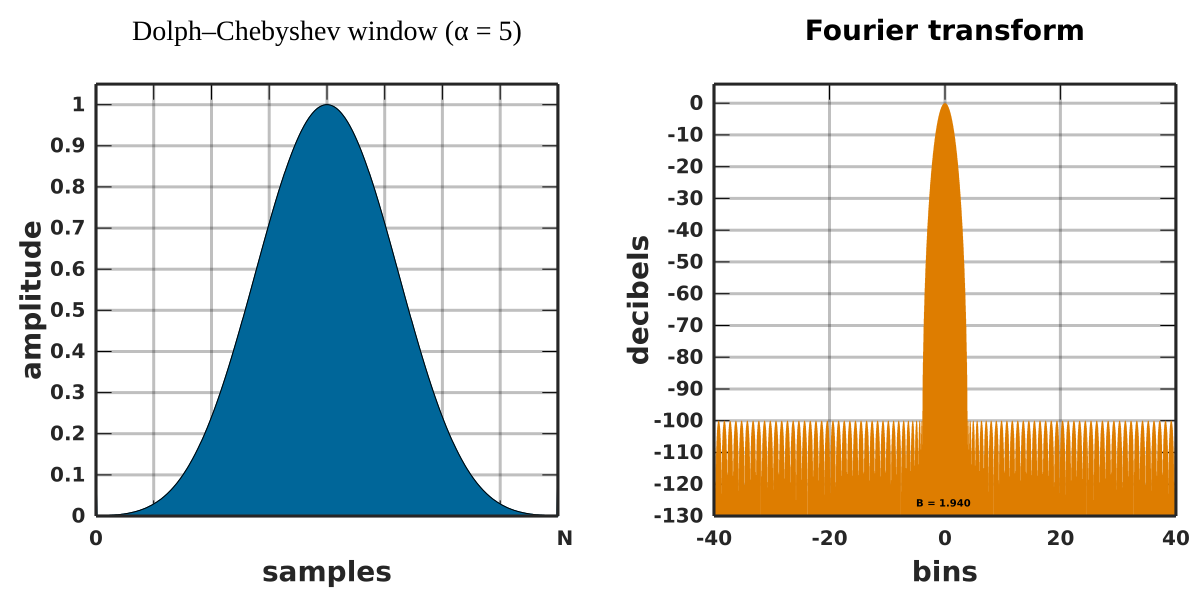
\includegraphics[width=\linewidth]{fig/window_dolph.png}
    \caption{Examples of the spectral leakage of some window functions}
    \label{fig:windowfunceffect}
\end{figure}

Zero-padding can be used to increase the number of output bins of the DFT. It is important to note that it does not increase the resolution of the DFT, it merely interpolates the coarse spectrum to become more smooth~\cite{zeropad1}. Two frequencies closer than $\Delta f_{bin}$ together will still fall in the same bin~\cite{zeropad2}. This form of interpolation is relatively compute intensive~\cite{interpolnozero}.

A less compute intensive method of interpolation is quadratic interpolation. It interpolates the actual location of a spectral peak between bins by fitting a quadratic function through the bins on a decibel scale~\cite{dbpolate, interpol}. We calculate a value $p \in [-\frac{1}{2}, \frac{1}{2}]$, which is the offset in bins of the interpolated peak with respect to the peak bin. Using the magnitude of the peak $y(0)$ and the magnitude of the neighbouring bins $y(-1)$ and $y(1)$, we define:
\begin{align*}
    \alpha &= 20 * {}^{10}\!\log{y(-1)} \\
    \beta  &= 20 * {}^{10}\!\log{y(0)} \\
    \gamma &= 20 * {}^{10}\!\log{y(1)}
\end{align*}
Then, we can calculate $p$ as follows:
\[ p = \frac{1}{2} \cdot \frac{\alpha - \gamma}{\alpha - 2\beta + \gamma} \]
The amplitude $a_i$ corresponding to the interpolated peak is:
\[ a_i = \beta - \frac{(\alpha - \gamma) * p}{4} \]
Given the bin number $b$ of the spectral peak location, the frequency $f_i$ corresponding to the interpolated peak is:
\[ f_i = \Delta f_{bin} * (b + p) \]
Quadratic interpolation can be combined with zero-padding for better results~\cite{interpolnozero}.

\subsection{Real-time}
Real-time is a difficult concept, as it has many definitions. Here are a few examples of relevant definitions:
\begin{enumerate}
    \item Being synced with actual clock time (or wall time). This is for instance relevant when playing media such as audio and video. When such media is played at an incorrect speed, it could be considered distorted. The hardware which keeps track of the clock time is called a real-time clock.
    \item A system must response within a specified time constraint, which is called the real-time constraint or deadline. This constraint is usually a relatively short time. This definition comes from real-time computing and is relevant when making car airbags or airplane control systems. Failing to response within the real-time constraint leads to failures of the system. Real-time systems are often classified into hard, firm and soft real-time based on the impact of missing the deadline~\cite{realclass}. Note that systems which have to respond seemingly instantaneous, such as graphical user interfaces or instant chatting/calling, are not real-time. There are no hard deadlines which the system has to respond within and the system does not fail if some delay does occur. Only user experience is slightly impacted.
    \item \textcolor{red}{A system which can process data faster than it acquires data.} This is technically not real-time, however, it is often used as such in academic literature. It is important for real-time system to process data faster than it acquires data so it does not lag behind after some time, however, this is an implicit deadline. Not having this deadline explicit may lead to non-sensible expectations of the system.
\end{enumerate}
Even though the first definition is very relevant when working with audio, it is not relevant for us. The audio drivers of operating systems handle all timing for us. We simply have to wait for samples to be recorded and made available to our program. We only have to keep the sampling rate in mind as shown in the previous section.

% TODO: Maybe it's a firm real-time system. And usefulness degrades more if latency was higher.
In order to allow guitarists to use their guitar as a MIDI instrument, our system has to respond within a small time frame. On top of that, if the system fails to respond quickly enough, the usefulness of the result degrades, as timing is very important when playing an instrument. These restrictions would classify our system as a soft real-time system. We choose a real-time of constraint of TODO milliseconds. We elaborate on this choice in section~\ref{sec:constraint}.

Other work in real-time pitch estimation often uses the third definition of real-time. This is a problem when using Fourier transform based methods, as many papers choose large frame sizes to get a high resolution in the frequency domain. For instance, in order to discern the two lowest notes on a guitar which are 4.9 Hz apart, we would need a frame length of 204 milliseconds. This is well over our real-time constraint and would be unplayable for any musician. Other papers which do explicitly set a real-time constraint, choose very high constraints from 140 ms~\cite{sloomboi} up to 360 ms~\cite{sloomboi2}. We have found no papers which choose a sensible real-time constraint.

\subsection{Music theory and notation}
In modern western music, we use the twelve-tone equal temperament (12-TET) music system. This system divides an octave, which is the interval between a pitch and another pitch with double the frequency, into twelve equally spaced semitones on the logarithmic scale. The logarithmic scale is used such that the perceived interval between two adjacent notes is constant~\cite{perception}. As a result, the ratio between two frequencies in an $n$-semitone interval is $\sqrt[12]{2}^n$ or $2^{\frac{n}{12}}$, invariant to pitch. A semitone further be divided into 100 logarithmically scales cents. Cents are often used to measure dissonance.

Using scientific pitch notation, every note can be uniquely identified by combining the traditional note names \note{A}{} to \note{G}{} (with accidentals such as $\sharp$ and $\flat$) with an octave number (e.g. \noteflat{E}{3}). An octave starts at \note{C}{}, which means the octave number increases between \note{B}{} and \note{C}{}. This counter intuitively implies \note{A}{3} is higher than \note{C}{3}. Note that in 12-TET, \notesharp{C}{} and \noteflat{D}{} are enharmonically equivalent. In this thesis, we will always refer to the sharp ($\sharp$) note instead of the enharmonically equivalent flat note ($\flat$). %Furthermore, even though technically \notesharp{B}{3} (which is equal to \note{C}{4}) is within the fourth octave, it is denoted to be in the third octave as accidentals do not change the octave number.
The range of a typical guitar in standard tuning is from \note{E}{2} up to \note{E}{6}.

The 12-TET music system only describes the relation between two notes in an interval. In order to play with other musicians in harmony, an arbitrary note has to be tuned to a specific frequency. Per ISO 16, the standard tuning frequency of the \note{A}{4} is 440 Hz within an accuracy of 0.5 Hz~\cite{isoa}.

Using the above information, we can translate frequencies into scientific note names and vice versa. In order to numerically work with note names, we assign a value to each note as shown in Table~\ref{tab:notenames}.
\begin{table}[H]
    \hfill
    \begin{center}
        \begin{tabular}{l|l}
            name & number \\
            \hline
            \note{C}{}      & 0 \\
            \notesharp{C}{} & 1 \\
            \note{D}{}      & 2 \\
            \notesharp{D}{} & 3 \\
            \note{E}{}      & 4 \\
            \note{F}{}      & 5
        \end{tabular}
        \qquad
        \begin{tabular}{l|l}
            name & number \\
            \hline
            \notesharp{F}{} & 6 \\
            \note{G}{}      & 7 \\
            \notesharp{G}{} & 8 \\
            \note{A}{}      & 9 \\
            \notesharp{A}{} & 10 \\
            \note{B}{}      & 11
        \end{tabular}
    \end{center}
    \hfill
    \caption{The number corresponding to each note name}
    \label{tab:notenames}
\end{table}
In order to make calculations easier, we use \note{C}{0} as a tuning note instead of \note{A}{4}. We can calculate the frequency of \note{C}{0} using the fact that \note{C}{0} is 57 semitones lower than \note{A}{4}:
\begin{align*}
    f_{C_0} = f_{A_4} * 2^{\frac{-57}{12}} &= 440 * 2^{\frac{-57}{12}} \\
                                           &= 16.352 \text{ Hz}
\end{align*}
% \[ f_{C_0} = 440 * 2^{\frac{-57}{12}} = 16.352 \text{ Hz} \]
% \[ 440 * \sqrt[12]{2}^{-57} = 16.352 Hz \]

We can calculate the frequency $f_{N_O}$, where $N$ is the note name which is represented by a numerical value given by Table~\ref{tab:notenames} and $O$ is the octave number using:
\begin{align*}
    f_{N_O} &= f_{C_0} * 2^O * 2^{\frac{N}{12}} \\
            &= f_{C_0} * 2^{O + \frac{N}{12}}
\end{align*}
% \[ f_{N_O} = f_{C_0} * 2^O * 2^{\frac{N}{12}} \]

To calculate the closest note $N_O$ corresponding to a frequency $f$, we first calculate the number of semitones $n_s$ between the tuning note $f_{C_0}$ and $f$:
\begin{align*}
    n_s = \round{12 * {}^{2}\!\log{\frac{f}{f_{C_0}}}}
\end{align*}
Here, $\round{\ldots}$ denotes rounding to the nearest integer. By rounding, we find the closest note to $f$. Now we can calculate $N$ and $O$ as follows:
\begin{align*}
    N &= n_s \mod 12 \\
    O &= \floor{\frac{n_s}{12}}
    % O &= n_s / 12
\end{align*}
Note that we assume $a \mod b$ always return a number $c$ for which $0 \leq c < b$. Some programming languages allow the modulo operator to return a value $c$ for which $-b < c < b$, resulting in $-13 \mod 10 = -3$ instead of $-13 \mod 10 = 7$. Furthermore, when using a conversion to an integer instead of a floor, the octave number is rounded up when the note distance is negative.

In order to calculate the error $e$ in cents of the given frequency to the closest tuned note, we first calculate the tuned frequency $f_t$ of the closest note:
\[ f_t = f_{C_0} * 2^{\frac{n_s}{12}} \]
Then the error $e$ can be calculated using:
\[ e = 1200 * {}^{2}\!\log{\frac{f}{f_t}} \]

\subsection{Envelope and transients}
The perceived loudness of a note over time can be described using an ADSR envelope. The ADSR envelope of a played note is the convex hull of the waveform of the signal, see Figure~\ref{fig:adsr} for an example. This convex hull can be divided in four parts: Attack, Decay, Sustain, Release. When a note is strummed on the guitar, a percussive sound is generated which causes a loud and sharp attack along with the note. This percussive sound quickly decays and only the actually fretted note will sustain. Finally, when the note is released, it dies out quickly.
\begin{figure}[H]
    \centering
    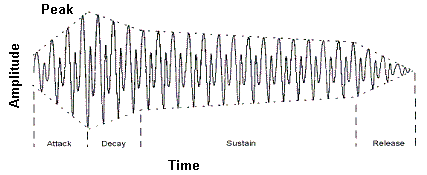
\includegraphics[width=\linewidth]{fig/envelope.png}
    \caption{Example of an ADSR envelope (TODO: Better image)}
    \label{fig:adsr}
\end{figure}

As mentioned before, when strumming a note, a percussive sound is generated. This sound is called a transient and contains a high degree of non-periodic components. Transients appear very chaotically in the frequency domain and thus is often considered as noise. Since a transient is of high amplitude, it overshadows the note which will eventually sustain. Because of this, we cannot use the samples from a transient for pitch estimation. This in turn increases our minimum latency, as we have to wait for samples which do not contain the transient any more.

\subsection{Fundamental frequency, overtones and timbre}  \label{sec:overtones}
When playing a note on an instrument, many sine waves are generated. The most notable frequency is called the fundamental frequency and determines what note is actually played. Integer multiples of the fundamental frequency can resonate and give rise to harmonic overtones~\cite{overtones}. In practice, these overtones are not exact integer multiples due to non-linear effect.

Furthermore, many other frequencies are generated along with the fundamental and its overtones. The instrument specific pattern of these frequencies, along with its envelope, is called the timbre of the instrument~\cite{timbre}. The timbre is what separates the sound of the same note played on two different instruments~\cite{perception}. Generally, the amplitude of the timbre frequencies is low compared to the fundamental frequency and can be disregarded as noise in the frequency domain.

In Section~\ref{sec:related}, we mentioned overtones are dissonant with respect to notes in 12-TET. This is true for all overtones, except for octaves, which are all overtones numbers equal to $2^n - 1$ for every $n$. In Table~\ref{tab:overseries}, we show an example for the overtones of \note{C}{4}. Note that the series of errors is the same, regardless of what the starting note is.
\begin{table}[H]
    \centering
    \begin{tabular}{rrcrr}
        $n$ & $f_{\text{overtone}}$ & closest note & $f_\text{note}$ & error \\
        \hline
        0 & 261.626  & $C_4$    & 261.626  &  - \\
        1 & 523.251  & $C_5$    & 523.251  &  0 \\
        2 & 784.877  & $G_5$    & 783.991  &  1.955 \\
        3 & 1046.502 & $C_6$    & 1046.502 &  0 \\
        4 & 1308.128 & $E_6$    & 1318.510 &  -13.686 \\
        5 & 1569.753 & $G_6$    & 1567.982 &  1.955 \\
        6 & 1831.379 & $A^\#_6$ & 1864.655 &  -31.174
    \end{tabular}
    \caption{Example of overtone series from \note{C}{4} and the errors compared to the closest note}
    \label{tab:overseries}
\end{table}
TODO: When using the CQT transform, none of the non-octave overtones coincides with a CQT bin, as the CQT bins are exponentially spaced like the notes in a scale. This causes the frequencies of the overtones to spread out over all other bins, resulting in more noise in the frequency domain. Furthermore, as shown in our research project, overtones are important for discerning fundamentals from noise generated by transients. By using a Fourier transform tuned to a specific note, all its overtones are also coincide with Fourier bins. By performing a Fourier tuned to every note in the 12 tone scale, we can accurately measure every note and its overtones. This gives us more accurate and information

TODO: The main problem in polyphonic pitch estimation comes from the occurrence of overtones. As mentioned before, notes in octave tend overshadow each other. Furthermore, as shown in Table~\ref{tab:overtones}, the overtones of a note can coincide with the...
TODO: Overtone overlap and polyphonic difficulty.
\begin{table}[H]
    \centering
    \hfill
    \begin{tabular}{r|l}
        $n$ & $f^{C_3}_0*n$ \\
        \hline
        1 & 130.813 \\
        2 & 261.626 \\
        \textcolor{red}{3} & \textcolor{red}{392.438} \\
        4 & 523.251 \\
        \textcolor{blue}{5} & \textcolor{blue}{654.064}
    \end{tabular}
    \hfill
    \begin{tabular}{r|l}
        $n$ & $f^{E_3}_0*n$ \\
        \hline
        1 & 164.814 \\
        2 & 329.628 \\
        3 & 494.441 \\
        \textcolor{blue}{4} & \textcolor{blue}{659.255} \\
        5 & 824.069
    \end{tabular}
    \hfill
    \begin{tabular}{r|l}
        $n$ & $f^{G_3}_0*n$ \\
        \hline
        1 & 195.998 \\
        \textcolor{red}{2} & \textcolor{red}{391.995} \\
        3 & 587.993 \\
        4 & 783.991 \\
        5 & 979.989
    \end{tabular}
    \hfill
    \caption{Overtones of C, E and G}
    \label{tab:overtones}
\end{table}
\begin{table}[H]
    \centering
    \begin{tabular}{c|c|c}
        Note & $f$ & $\Delta f$ \\
        \hline
        $f^{C_3}_2$ & 392.438 & \multirow{2}{*}{0.443} \\
        $f^{G_3}_1$ & 391.995 & \\
        \hline
        $f^{C_3}_4$ & 654.064 & \multirow{2}{*}{5.191} \\
        $f^{E_3}_3$ & 659.255 &
    \end{tabular}
    \caption{Colliding overtones}
    \label{tab:diff}
\end{table}


\section{Thesis content}
\textcolor{gray}{Actual research etc. Summary what was done in the research project which we build on. Notes on future work of research project.}

\textcolor{gray}{As mentioned in Section~\ref{sec:related} and shown in our research project, the resolution in the frequency domain is not sufficient for spectral peak selecting methods. Given the info in preliminaries, we can tune Fouriers to specific frequencies.}

\subsection{Real-time constraint}  \label{sec:constraint}
\textcolor{gray}{Start with the factors coming into play when choosing the real-time constraint for our system (latency, played notes per second etc). Note on measured latency in Appendix~\ref{sec:ax100}. Empirically found bounds on latency using our latency program}

\subsection{Software amplification}
\textcolor{gray}{(Software representation of samples and FFT). The FFT works on floating point numbers but most audio interfaces give up to 24 bit integers...}
\textcolor{gray}{We found empirically that when amplifying the input signal in software, peaks in the frequency domain are much easier to detect. However, it has to be done carefully to prevent distortion artifacts.}

\subsection{Parallel Fourier transforms}


\section{Implementation}
\textcolor{gray}{Details about the program I've written. Usage instructions, code choices, code structure, screenshots, expandability}



\section{Experiments}  \label{sec:exp}
\textcolor{gray}{Note that the parameters were empirically optimized with informal experiments. Datasets. Actual experiments.}


\section{Conclusions}
\textcolor{gray}{What we did in this thesis. Reflection on the performance of the system. Final reference to the source code.}


\section{Future work}  \label{sec:future}
\textcolor{gray}{What could still be improved/further researched.}



\appendix
\section{Measuring the latency of the AXON AX 100 mkII}  \label{sec:ax100}
\textcolor{gray}{Lekker meten en weten.}

\section{Effect of different window functions}
\textcolor{gray}{Plots met effect van verschillende window functions.}


\addcontentsline{toc}{section}{Bibliography}
\bibliographystyle{plain}
% \bibliographystyle{alpha}
\bibliography{thesis}

\end{document}
 